% !TEX root = ../main.tex
\begin{document}

\section{ソフトウェアテストの結果について}
入力内容と期待される出力内容を表\ref{入力内容と期待される出力内容}に示す。
\begin{table}[H]
    \centering
    \caption{入力内容と期待される出力内容}
    \label{入力内容と期待される出力内容}
\end{table}
\begin{longtable}{|c|c|c|c|} % \hline
    \hline
    入力内容 & 期待される出力内容 & 実際の出力内容 & 期待される結果と実際の結果の比較 \\ \hline
    \endfirsthead
    \hline
    入力内容 & 期待される出力内容 & 実際の出力内容 & 期待される結果と実際の結果の比較 \\ \hline
    \endhead
    % \hline
    \endfoot

    1
        &
            \begin{tabular}{c}
                0 \\
                0 \\
                0 \\
                0 \\
                0 \\
                0 \\
                0 \\
                0 \\
                0 \\
                0 \\
            \end{tabular}
        &
            \begin{tabular}{c}
                0 \\
                0 \\
                0 \\
                0 \\
                0 \\
                0 \\
                0 \\
                0 \\
                0 \\
                0 \\
            \end{tabular}
            
        & 成功 \\ \hline
    1371
        &
            \begin{tabular}{c}
                8796 \\
                3696 \\
                6604 \\
                6128 \\
                5523 \\
                5035 \\
                3512 \\
                3341 \\
                1622 \\
                6308 \\
            \end{tabular}
        &
            \begin{tabular}{c}
                8796 \\
                3696 \\
                6604 \\
                6128 \\
                5523 \\
                5035 \\
                3512 \\
                3341 \\
                1622 \\
                6308 \\
            \end{tabular}
        & 成功 \\ \hline
    2639
        &
            \begin{tabular}{c}
                9643 \\
                9874 \\
                4958 \\
                5817 \\
                8374 \\
                1238 \\
                5326 \\
                3662 \\
                4102 \\
                8264 \\
            \end{tabular}
        &
            \begin{tabular}{c}
                9643 \\
                9874 \\
                4958 \\
                5817 \\
                8374 \\
                1238 \\
                5326 \\
                3662 \\
                4102 \\
                8264 \\
            \end{tabular}
        & 成功 \\ \hline
    6174
        &
            \begin{tabular}{c}
                1182 \\
                3971 \\
                7688 \\
                1053 \\
                1088 \\
                1837 \\
                3745 \\
                250 \\
                625 \\
                3906 \\
            \end{tabular}
        &
            \begin{tabular}{c}
                1182 \\
                3971 \\
                7688 \\
                1053 \\
                1088 \\
                1837 \\
                3745 \\
                250 \\
                625 \\
                3906 \\
            \end{tabular}
        & 成功 \\ \hline
    8738
        &
            \begin{tabular}{c}
                3526 \\
                4326 \\
                7142 \\
                81 \\
                65 \\
                42 \\
                17 \\
                2 \\
                0 \\
                0 \\
            \end{tabular}
        &
            \begin{tabular}{c}
                3526 \\
                4326 \\
                7142 \\
                81 \\
                65 \\
                42 \\
                17 \\
                2 \\
                0 \\
                0 \\
            \end{tabular}
        & 成功 \\ \hline
    9172
        &
            \begin{tabular}{c}
                1255 \\
                5750 \\
                625 \\
                3906 \\
                2568 \\
                5946 \\
                3549 \\
                5954 \\
                4501 \\
                2590 \\
            \end{tabular}
        &
            \begin{tabular}{c}
                1255 \\
                5750 \\
                625 \\
                3906 \\
                2568 \\
                5946 \\
                3549 \\
                5954 \\
                4501 \\
                2590 \\
            \end{tabular}
        & 成功 \\ \hline
    9999
        &
            \begin{tabular}{c}
                9800 \\
                400 \\
                1600 \\
                5600 \\
                3600 \\
                9600 \\
                1600 \\
                5600 \\
                3600 \\
                9600 \\
            \end{tabular}
        &
            \begin{tabular}{c}
                9800 \\
                400 \\
                1600 \\
                5600 \\
                3600 \\
                9600 \\
                1600 \\
                5600 \\
                3600 \\
                9600 \\
            \end{tabular}
        & 成功 \\ \hline
\end{longtable}
% \end{table}

以下にプログラムの実行結果を示す。

% \lstinputlisting[label=実行結果, caption=実行結果,]{./main_result.txt}
\begin{figure}[H]
    \centering
    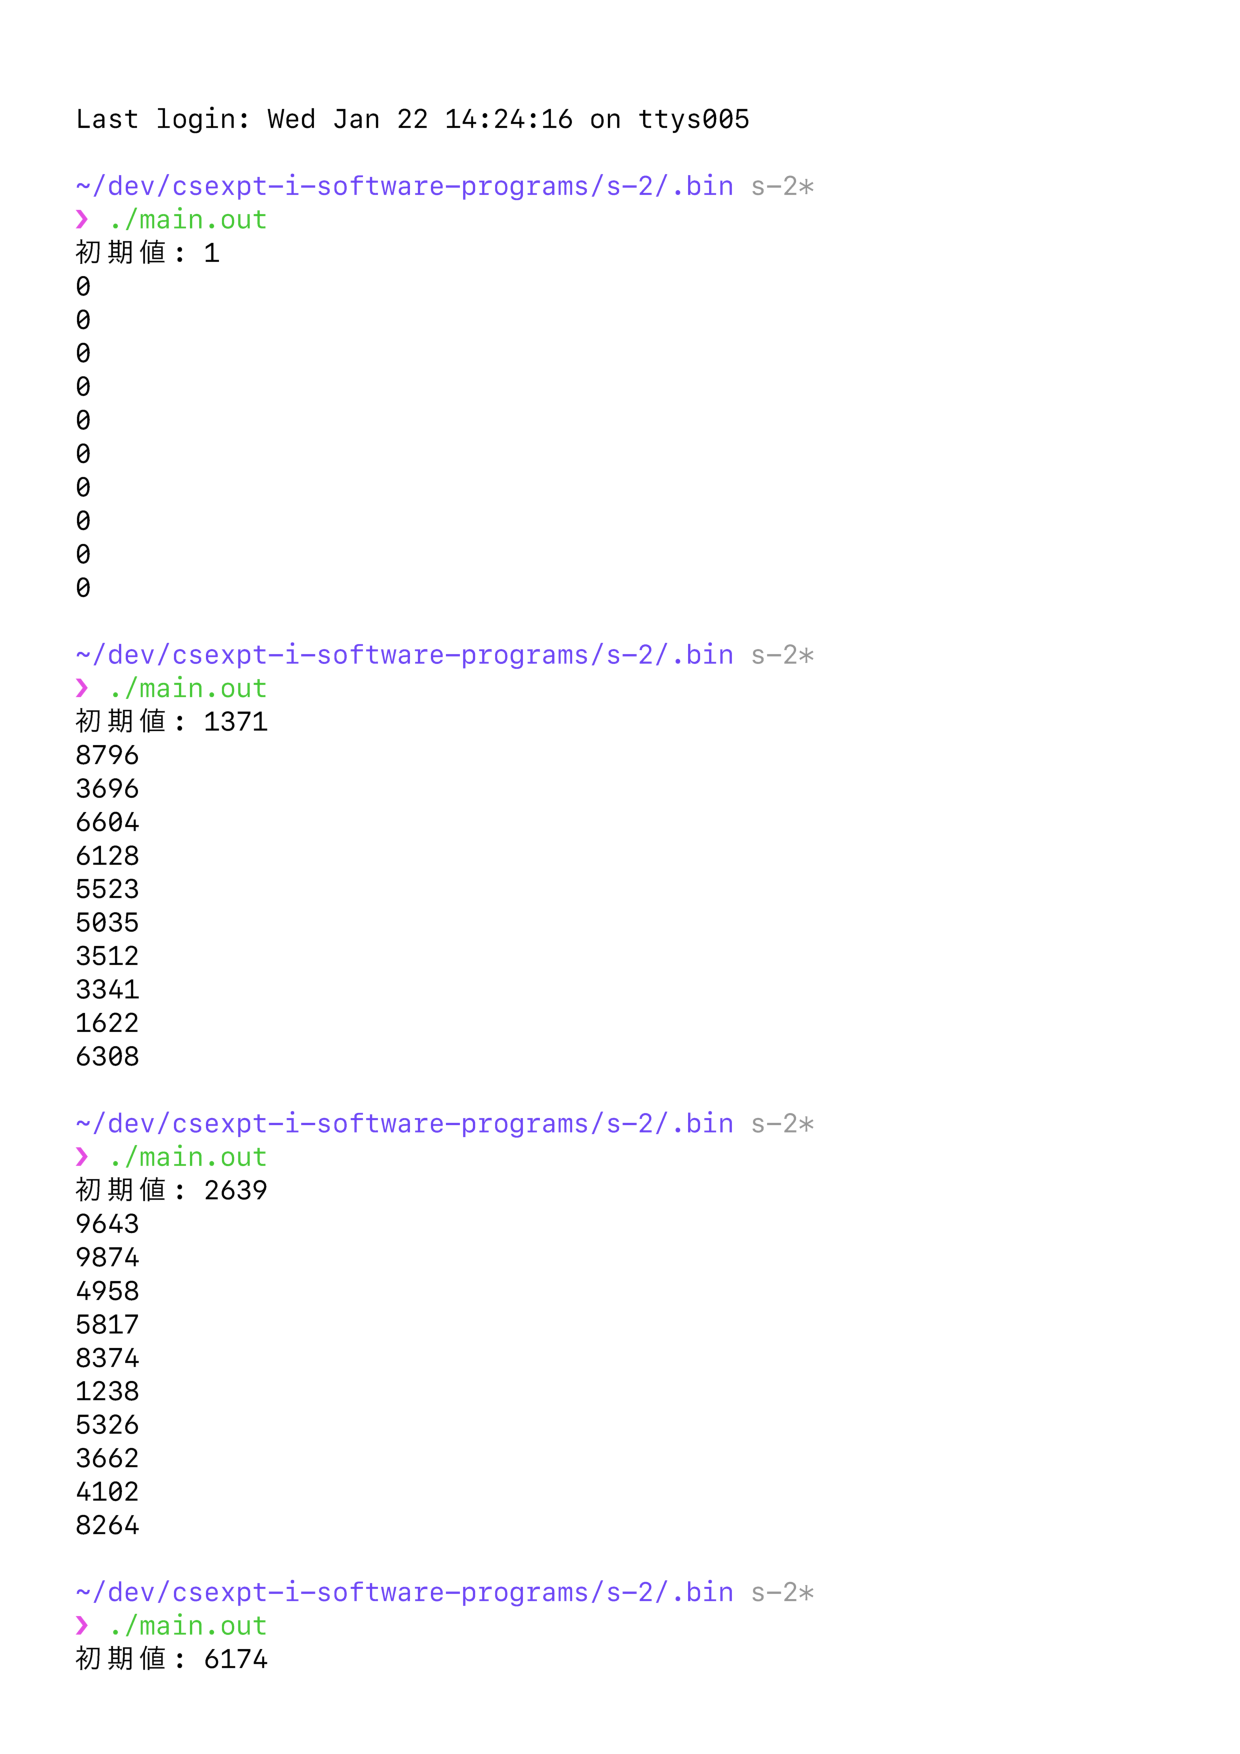
\includegraphics[width=0.8\hsize, pagebox=mediabox, page=1]{main_result_img.pdf}
    \caption{実行結果}
    \label{実行結果}
\end{figure}
\begin{figure}[H]
    \ContinuedFloat
    \centering
    \includegraphics[width=0.8\hsize, pagebox=mediabox, page=2]{main_result_img.pdf}
    \caption{実行結果}
    \label{実行結果}
\end{figure}
\begin{figure}[H]
    \ContinuedFloat
    \centering
    \includegraphics[width=0.8\hsize, pagebox=mediabox, page=3]{main_result_img.pdf}
    \caption{実行結果}
    \label{実行結果}
\end{figure}

表\ref{入力内容と期待される出力内容}の結果より、期待された出力を行っているから、プログラムリスト\ref{作成したプログラム}は正しい。

\subsection{オプションのソフトウェアテストの結果について}

プログラムリスト\ref{作成したプログラム}の11行目の $n < 10$ を $n < 100$ に変えることで100個の擬似乱数の生成を行うことができる。そのプログラムに入力$6174$を与えた時の実行結果を示す。

% \lstinputlisting[label=10以上の出力を行う実行結果, caption=10以上の出力を行う実行結果]{./option_result.txt}
\begin{figure}[H]
    \centering
    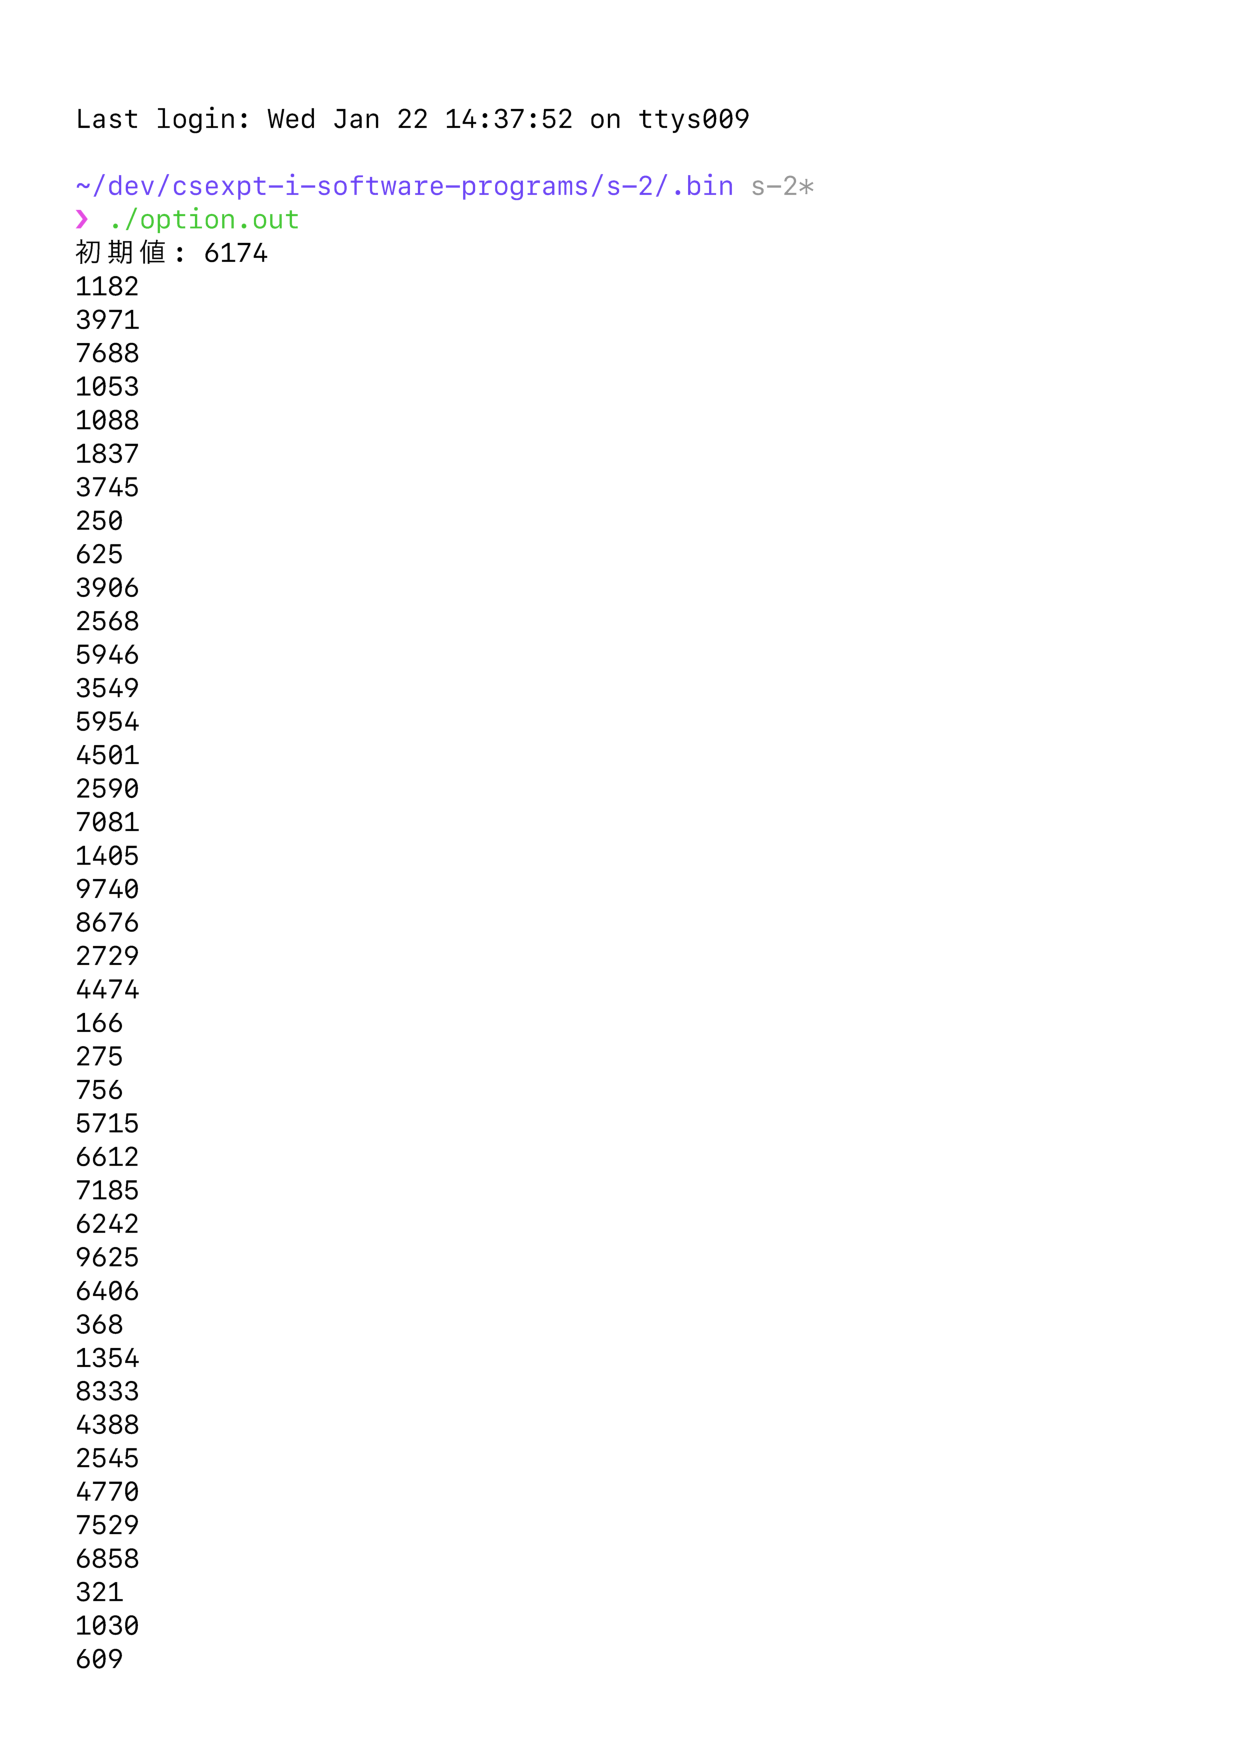
\includegraphics[width=0.8\hsize, pagebox=mediabox, page=1]{option_result_img.pdf}
    \caption{10以上の出力を行う実行結果}
    \label{10以上の出力を行う実行結果}
\end{figure}
\begin{figure}[H]
    \ContinuedFloat
    \centering
    \includegraphics[width=0.8\hsize, pagebox=mediabox, page=2]{option_result_img.pdf}
    \caption{10以上の出力を行う実行結果}
    \label{10以上の出力を行う実行結果}
\end{figure}
\begin{figure}[H]
    \ContinuedFloat
    \centering
    \includegraphics[width=0.8\hsize, pagebox=mediabox, page=3]{option_result_img.pdf}
    \caption{10以上の出力を行う実行結果}
    \label{10以上の出力を行う実行結果}
\end{figure}

以上の実行結果により、一度100の倍数である数字が乱数の生成結果となると、次の乱数の下2桁は必ずゼロとなってしまい、さらにその結果が繰り返されることがわかった。
初期値に100の倍数を与えた実行結果を次に示す。

% \lstinputlisting[label=初期値に100の倍数を与えた時の実行結果, caption=初期値に100の倍数を与えた時の実行結果]{./main_result2.txt}
\begin{figure}[H]
    \centering
    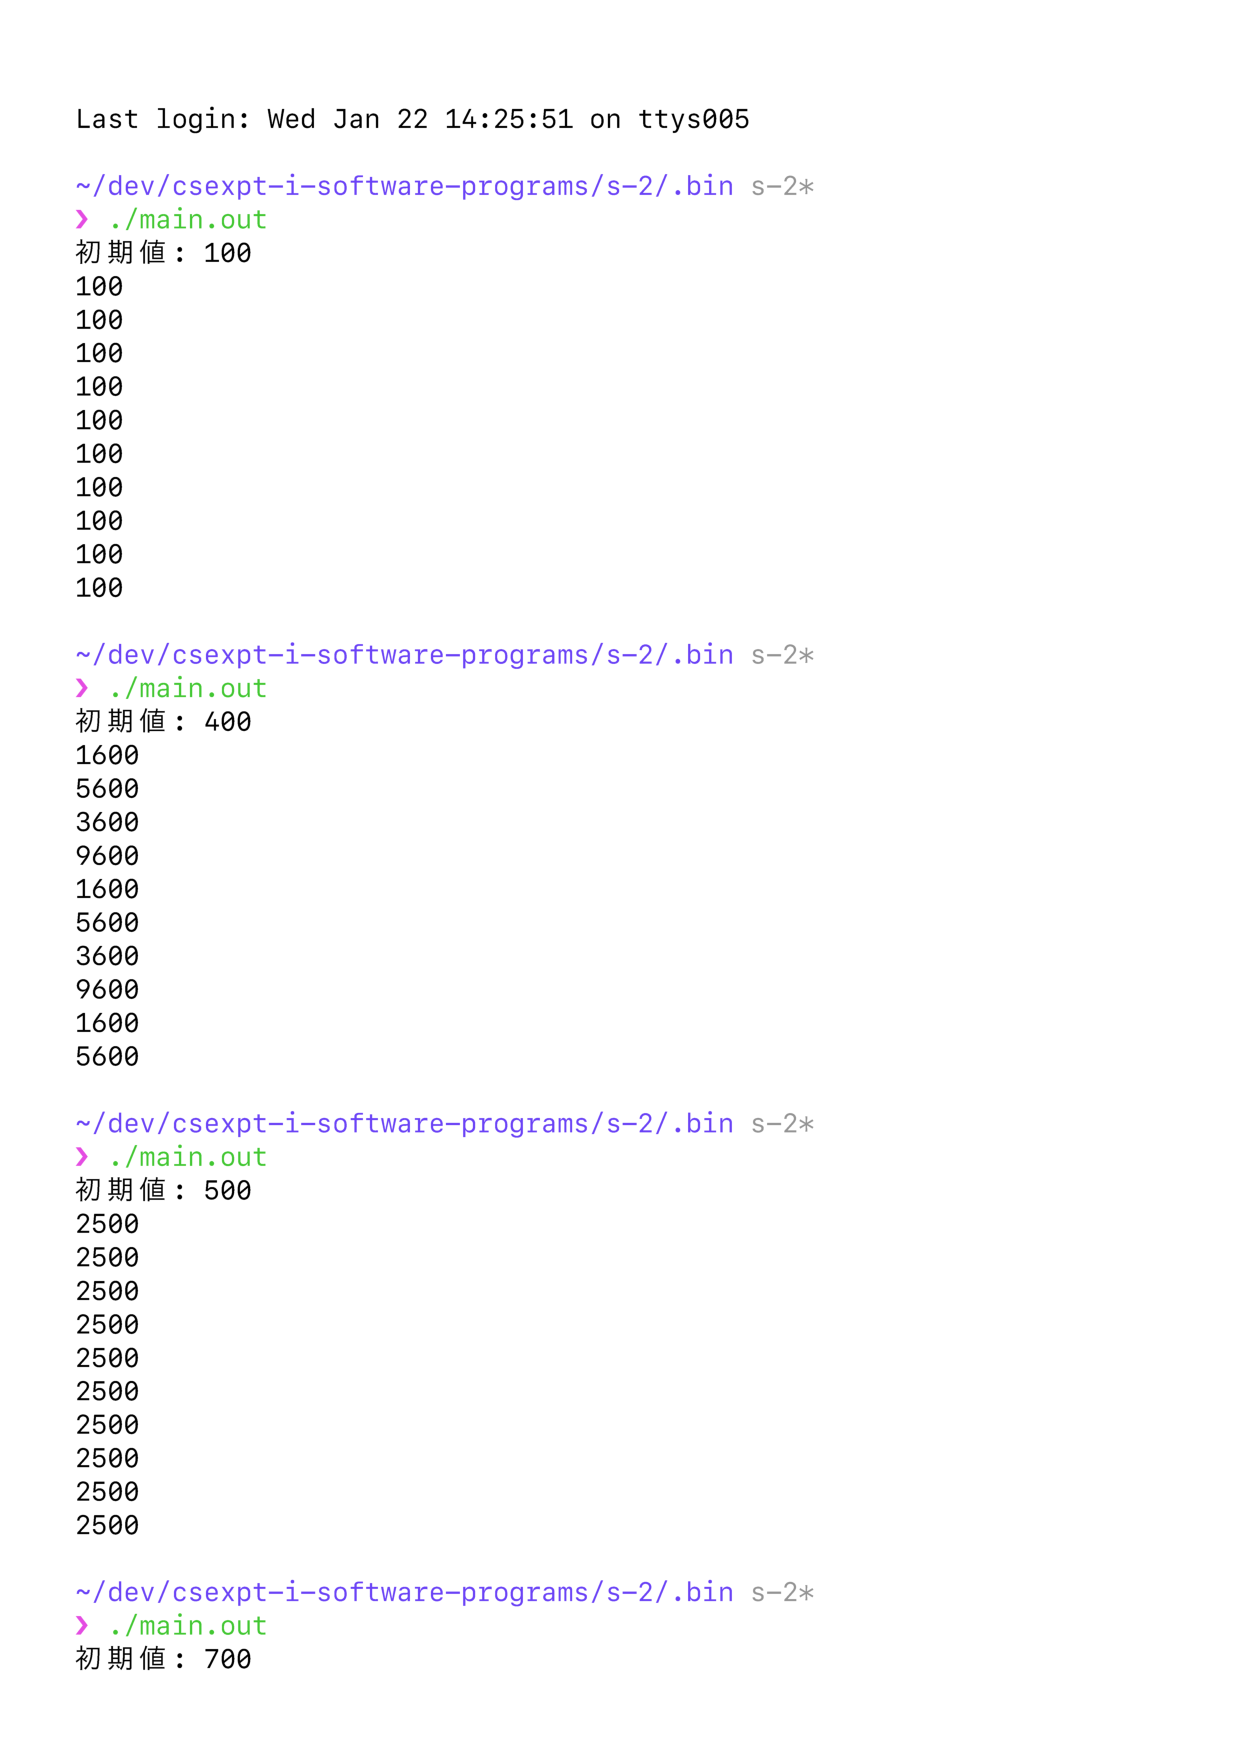
\includegraphics[width=0.8\hsize, pagebox=mediabox, page=1]{main_result2_img.pdf}
    \caption{初期値に100の倍数を与えた時の実行結果}
    \label{初期値に100の倍数を与えた時の実行結果}
\end{figure}
\begin{figure}[H]
    \ContinuedFloat
    \centering
    \includegraphics[width=0.8\hsize, pagebox=mediabox, page=2]{main_result2_img.pdf}
    \caption{初期値に100の倍数を与えた時の実行結果}
    \label{初期値に100の倍数を与えた時の実行結果}
\end{figure}
\begin{figure}[H]
    \ContinuedFloat
    \centering
    \includegraphics[width=0.8\hsize, pagebox=mediabox, page=3]{main_result2_img.pdf}
    \caption{初期値に100の倍数を与えた時の実行結果}
    \label{初期値に100の倍数を与えた時の実行結果}
\end{figure}

また表\ref{入力内容と期待される出力内容}の$8738$の結果より、100未満の数を与えた場合に、生成を繰り返すと$0$になると仮定する。

% \lstinputlisting[label=初期値に100未満の数与えた時の実行結果, caption=初期値に100未満の数を与えた時の実行結果]{./main_result3.txt}
\begin{figure}[H]
    \centering
    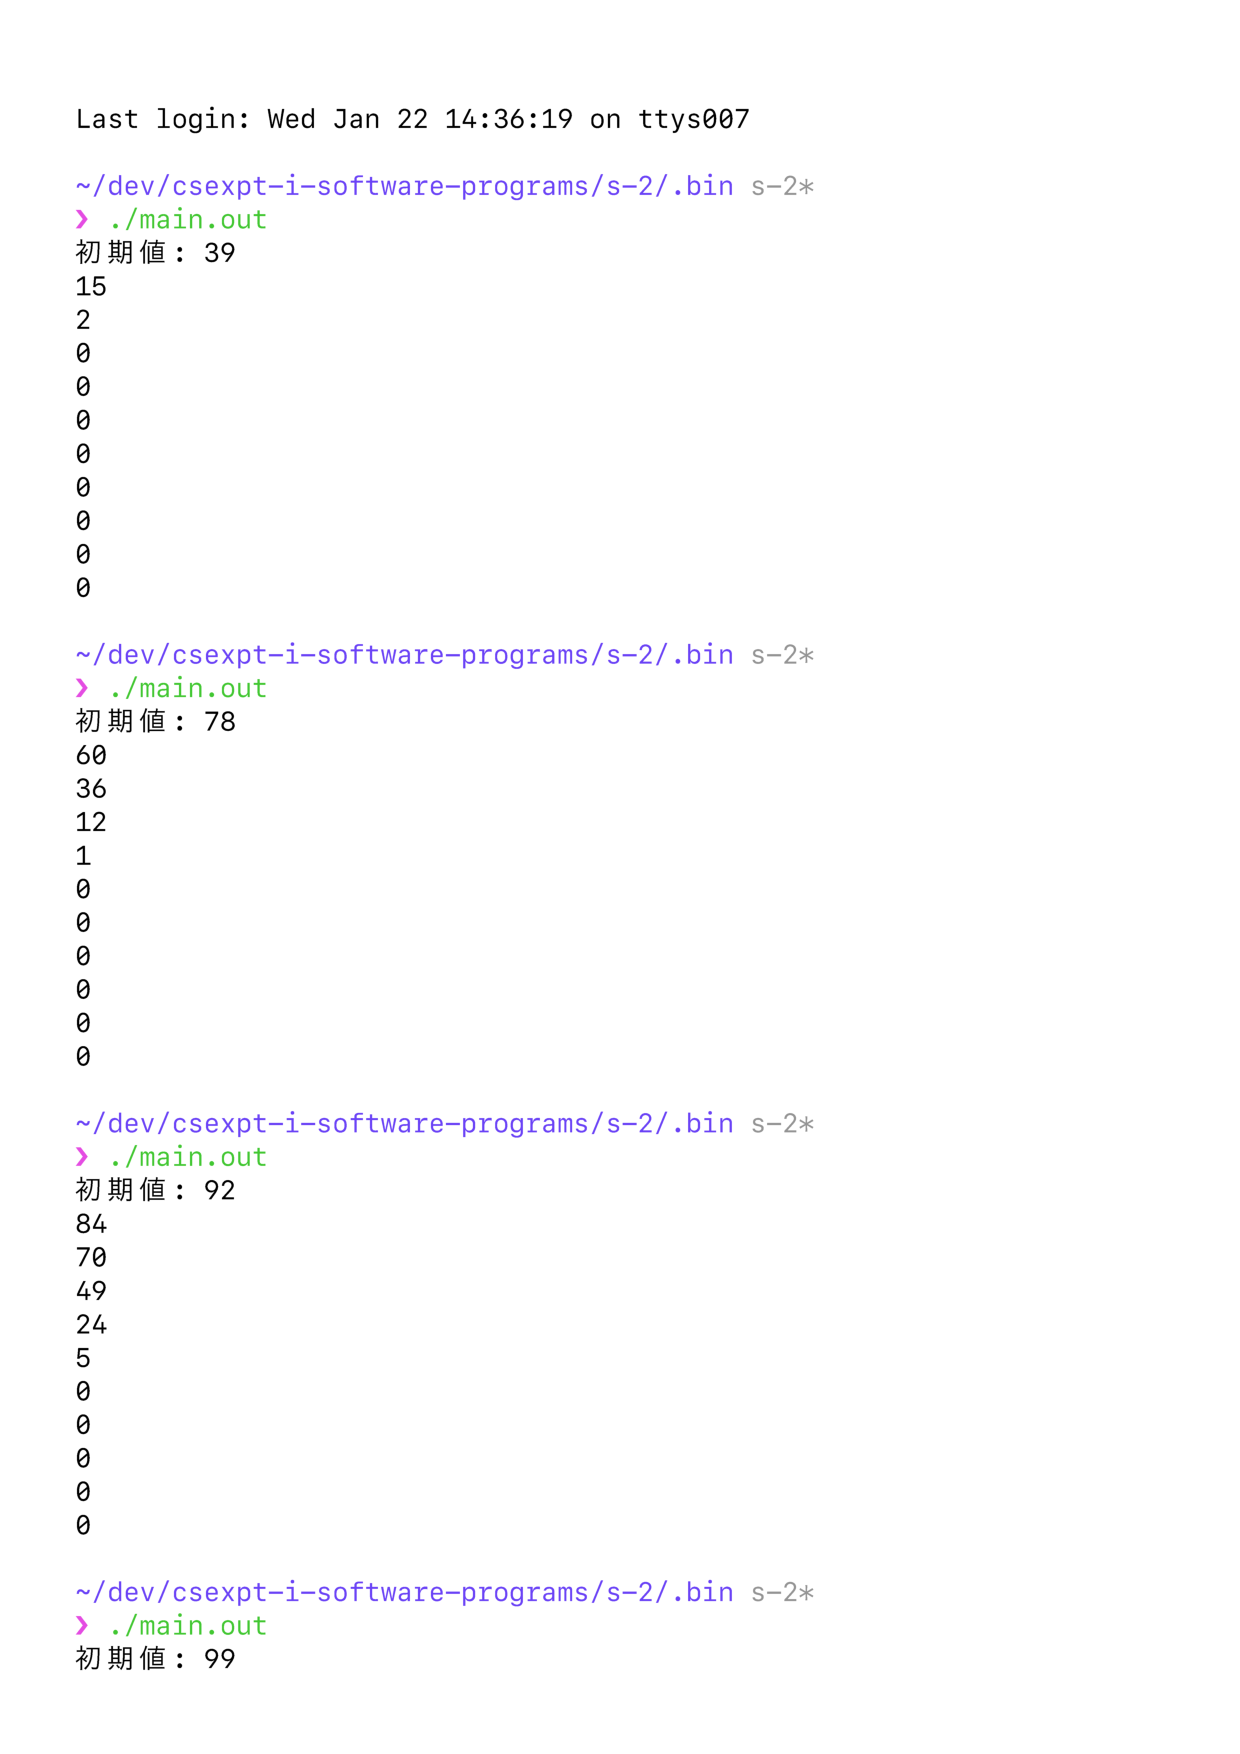
\includegraphics[width=0.8\hsize, pagebox=mediabox, page=1]{main_result3_img.pdf}
    \caption{初期値に100未満の数与えた時の実行結果}
    \label{初期値に100未満の数与えた時の実行結果}
\end{figure}
\begin{figure}[H]
    \ContinuedFloat
    \centering
    \includegraphics[width=0.8\hsize, pagebox=mediabox, page=2]{main_result3_img.pdf}
    \caption{初期値に100未満の数与えた時の実行結果}
    \label{初期値に100未満の数与えた時の実行結果}
\end{figure}

$n < 100$ のとき、$n^2$ は必ず $n^2 < 10000$ となる。この結果の上2桁は元の$n$よりも小さくなる。したがって、100未満の数を与えた時、必ず値が減少していくことから、10未満になる。
さらに生成を進めると、10未満の時の自乗の結果は必ず100未満であるから、上2桁を取り出すと$0$となる。よって、この先の生成では$0$が繰り返される。

以上より、乱数の生成過程において、100の倍数および100未満の数が結果となる場合、100の倍数および100未満の数を与えた場合に乱数としての結果が期待できないことから、この方法が使われなくなったと考えられる。
\end{document}